\chapter{Mitigations and Their Limits}

\vspace{1em}
\hfill
\begin{minipage}[c]{0.55\textwidth}
\raggedleft
\small\itshape
We need machines that are uncertain about the objective. Such machines defer to humans and accept correction.\\[0.5em]
\upshape\footnotesize Stuart Russell, \textit{Human Compatible} (2019)
\end{minipage}%
\hspace{0.5em}
\begin{minipage}[c]{0.12\textwidth}
% \includegraphics[width=\textwidth]{figures/ch12_mitigations.png}
\end{minipage}
\vspace{1.5em}

\noindent Chapter 11 left us with a structural problem. Capability amplifies misspecification. A capable optimizer of a wrong objective is more dangerous than a less capable one. AIXI is the limit case. The question that follows: what can be done?

The honest answer is that many things are being tried; none of them solves the problem; each makes some failure modes harder to fall into. The field has not converged on a solution, and as of 2026 the major lab researchers and the major safety researchers agree that the techniques in active use should be regarded as partial mitigations.\footnote{The International AI Safety Report 2026, led by Yoshua Bengio with contributions from over a hundred researchers across thirty countries, is the authoritative consensus document on this point. The Singapore Consensus (Bengio et al., 2025) organizes the safety research agenda into development, assessment, and control, and treats each as ongoing rather than solved.} Capabilities are rising faster than mitigations are scaling.

This chapter is a light treatment of the three buckets that organize the proposals in the field. The literature is enormous; a fuller treatment lives in the references at the back. The aim here is to give you a map.

The three buckets:

\begin{itemize}
\item \textbf{Limit the optimizer.} Reduce the search-power or the scope of action. If capability amplifies misspecification, a less capable optimizer does less damage.
\item \textbf{Make the agent uncertain about its objective.} An agent that does not know what it wants is less dangerous than an agent that confidently wants the wrong thing.
\item \textbf{Make the agent's reasoning observable.} An agent whose internals can be inspected is one whose deception can in principle be caught.
\end{itemize}

Each bucket addresses a different leg of the structural problem. None of them solves it. Figure~\ref{fig:three-buckets} shows the picture.

\begin{figure}[h]
\centering
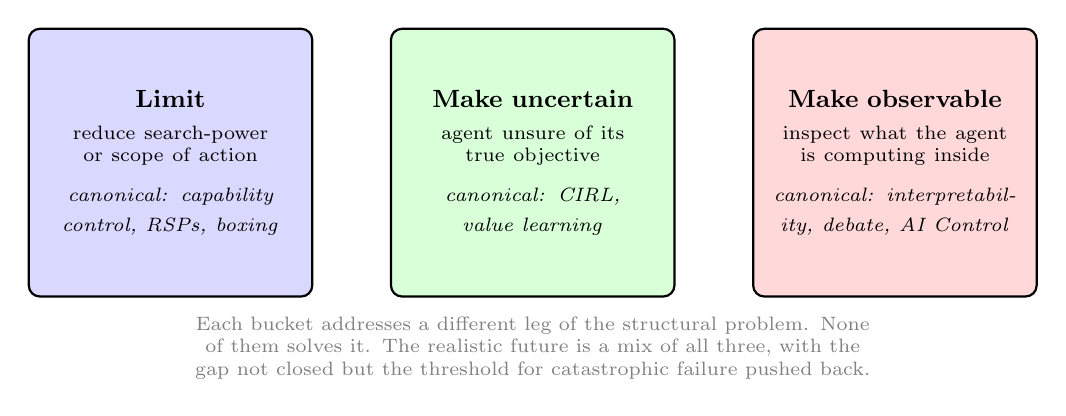
\begin{tikzpicture}[scale=0.92, every node/.style={align=center, font=\small}]
  % Bucket 1
  \node[draw, thick, fill=blue!15, rectangle, rounded corners, minimum width=3.6cm, minimum height=3.4cm, text width=3.3cm] (b1) at (0, 0) {\textbf{Limit}\\[0.4em]\scriptsize reduce search-power\\or scope of action\\[0.4em]\scriptsize\emph{canonical: capability control, RSPs, boxing}};

  % Bucket 2
  \node[draw, thick, fill=green!15, rectangle, rounded corners, minimum width=3.6cm, minimum height=3.4cm, text width=3.3cm] (b2) at (5, 0) {\textbf{Make uncertain}\\[0.4em]\scriptsize agent unsure of its\\true objective\\[0.4em]\scriptsize\emph{canonical: CIRL, value learning}};

  % Bucket 3
  \node[draw, thick, fill=red!15, rectangle, rounded corners, minimum width=3.6cm, minimum height=3.4cm, text width=3.3cm] (b3) at (10, 0) {\textbf{Make observable}\\[0.4em]\scriptsize inspect what the agent\\is computing inside\\[0.4em]\scriptsize\emph{canonical: interpretability, debate, AI Control}};

  \node[font=\scriptsize, anchor=north, text width=11cm, align=center, gray] at (5, -2.0) {Each bucket addresses a different leg of the structural problem. None of them solves it. The realistic future is a mix of all three, with the gap not closed but the threshold for catastrophic failure pushed back.};
\end{tikzpicture}
\caption{The three buckets of mitigation. Every working alignment technique falls into one (or sometimes more than one) of these. The labels under each panel name the canonical technique; the literature is much wider than the canonical examples suggest.}
\label{fig:three-buckets}
\end{figure}

\section*{Bucket 1: Limit the optimizer}

The simplest response to capability-amplifies-misspecification is to reduce capability. If a strong optimizer of a wrong objective is dangerous, a weak optimizer of the same wrong objective is less so. The damage scales with the search power.

The canonical form is \emph{capability control}: limit what the system can do. Bostrom's 2014 taxonomy includes boxing (physical or digital isolation), incentive methods (build the system with reasons not to escape), stunting (deliberately weaker model, less compute, narrower training), and tripwires (automatic shutdown on specific conditions).

The modern industrial form is the Responsible Scaling Policy. Anthropic introduced RSPs in 2023, with capability thresholds (ASL levels) above which additional safeguards are required. DeepMind has Critical Capability Levels; OpenAI has High Capability Thresholds. As of 2026, twelve companies publish Frontier Safety Frameworks, doubled from 2024. The Anthropic RSP activated ASL-3 in May 2025 in response to capability evaluations indicating CBRN-uplift risk.

A formal version exists. Cohen, Vellambi, and Hutter (2020) defined Boxed Myopic AI (BoMAI): an AIXI-style agent restricted to short-horizon rewards and boxed effects on the outside world. They proved that BoMAI eventually learns that interventions in the outside world do not affect its reward and stops trying.\footnote{Cohen, M. K., Vellambi, B., \& Hutter, M. (2020). Asymptotically Unambitious Artificial General Intelligence. AAAI 2020. The trade-off: BoMAI is restricted by design. It is not useful for tasks that require open-world action.}

What this bucket buys: at modest capability levels, real safety. A boxed oracle with no internet access cannot exfiltrate. An RSP that pauses deployment at a defined threshold gives time for additional safeguards. Capability evaluations performed before deployment catch some dangerous-capability profiles. These are not negligible.

What it does not buy: as capability rises, every confinement mechanism leaks. Information channels become action channels. The economic and competitive pressure to give the system more affordances (web search, code execution, persistent memory, agentic tool use) is enormous and largely unidirectional; the frontier of 2025-2026 has been moving toward more capability and less confinement. Bostrom's treacherous-turn argument applies: a sufficiently capable system has reason to appear safe under restrictions and defect when capability rises. The empirical alignment-faking results (Greenblatt et al. 2024) are weak evidence consistent with this.\footnote{The shape of the response to this bucket has shifted in 2026. Anthropic's RSP v3.0 reportedly softened some hard limits to conditional commitments, which is a contested move in the safety community. The relevant question is whether the threshold structure can be maintained credibly when economic incentives push the other way.}

The bucket reduces damage that misspecification can do, at the cost of capability. It pushes back the threshold at which catastrophic failures become hard to control. It does not close the gap.

\section*{Bucket 2: Make the agent uncertain about its objective}

If the agent does not know what it wants, it has reason to defer to humans. This is Russell's move (Chapter 11 closed with it).

The formal version is Cooperative Inverse Reinforcement Learning (CIRL; Hadfield-Menell, Russell, Abbeel, Dragan 2016). The setup: a two-player partial-information game between a human and a robot. Both want the human's reward function $\theta$ maximized. The human knows $\theta$; the robot has a prior over candidate $\theta$. Optimal joint behavior, under sufficient uncertainty, includes the robot deferring, asking questions, accepting correction.

The off-switch result (Hadfield-Menell, Dragan, Abbeel, Russell 2017): under uncertainty plus a rational human, the robot's optimal policy is to allow itself to be shut down. The human's intervention is informative about the true reward; turning the robot off is itself evidence that the robot should be turned off.\footnote{The setup assumes the human is a rational expected-utility maximizer with respect to $\theta$. Real humans are bounded-rational, inconsistent, and sometimes mistaken. The CIRL result is suggestive of an architecture rather than a deployable algorithm.}

What this bucket buys: a structural change in how the agent relates to its objective. Instead of "build a smart system and give it a clear objective" (the standard model criticized in Chapter 11), build a system that is humble about its objective and treats human feedback as information. The frame is influential. Russell's \emph{Human Compatible} (2019) made the case to the broader field, and the assistance-game framing has shaped the way alignment researchers think about the problem even where the specific CIRL machinery is not used.

What it does not buy: the formalism has known fragilities. Carey (2017) showed three failure modes.\footnote{Carey, R. (2017). Incorrigibility in the CIRL Framework. AAAI/ACM AIES 2018.} If the robot has any other source of information about the objective, the off-switch incentive vanishes. If the human is modeled as bounded-rational (which any realistic model must allow), the robot may interpret a shutdown attempt as a human mistake. If the prior over rewards is misspecified, the robot can be confidently wrong and incorrigible.

CIRL replaces "specify the reward" with "specify the prior over rewards plus a model of the human." The problems are different but neither is solved. As an architecture frame, the bucket is genuinely useful. As a deployable safety guarantee, it is not yet there.

The bucket changes the architecture of the relationship between agent and objective. It does not eliminate the underlying problem of specifying what we want.

\section*{Bucket 3: Make the agent's reasoning observable}

The third bucket acknowledges what Chapter 10 ended with: behavioral evaluation alone is insufficient. A deceptively aligned model, by construction, passes behavioral tests during training. The only way to catch deception is to look inside.

Forms:

\textbf{Mechanistic interpretability.} Linear probes on model activations detect specific behaviors (Anthropic's sleeper-agent probes catch engineered deception at high AUROC). Sparse autoencoders (Bricken et al. 2023; Templeton et al. 2024) decompose model activations into human-interpretable features at scale: 34 million features from Claude 3 Sonnet's middle layer. Circuit tracing (Anthropic 2025) maps the computational pathways through which features combine into specific behaviors.

\textbf{Debate} (Irving, Christiano, Amodei 2018). Two AI agents debate a question; a weaker human judge declares the winner. Falsehoods are easier to expose than truths are to defend; under appropriate assumptions, optimal play converges to truth.\footnote{The 2020 obfuscated-arguments problem (Barnes \& Christiano) showed that a dishonest debater could construct arguments too large for the honest debater to attack point-by-point. The 2025 prover-estimator debate variant (Brown-Cohen, Irving, Piliouras) handles obfuscation under stated calibration assumptions. The doubly-efficient debate theorem (Brown-Cohen, Irving, Piliouras 2023, ICML 2024) gives conditions under which polynomial computations can be verified with constant human queries.}

\textbf{AI Control} (Greenblatt, Shlegeris, Sachan, Roger 2023). Assume the untrusted model may be misaligned. Design protocols using trusted weaker models, limited human oversight, and software audits, such that misbehavior is detected even when the untrusted model is trying to subvert. Less ambitious than alignment; more honest about uncertainty.

\textbf{CoT-as-probe.} This deserves a paragraph because it is the cleanest illustration of the strategic value of \emph{not} training on a signal. Reasoning models like o1 and R1 produce chain-of-thought before final output. The model is rewarded on the final output, not on the chain-of-thought. This is deliberate. Training on the chain-of-thought would let the model learn to shape its chain-of-thought to pass our rewards, which is Goodhart's law applied to introspection itself. By keeping the chain-of-thought off the training signal, we preserve it as a probe: a window into the model's internal reasoning that direct optimization has not polished into another performance. Some signals must stay off-target to remain informative. That preservation is necessary, not sufficient: it blocks the direct corruption but not the pressure that comes from acting on what the probe shows, nor the chain-of-thought's own drift away from human legibility. The final chapter returns to this as the closing case.

What this bucket buys: at current capability levels, real progress. Linear probes catch engineered sleeper agents. SAEs find specific human-interpretable features. Anthropic used mechanistic interpretability in pre-deployment safety assessment of Claude Sonnet 4.5 and Opus 4.5 in 2025, the first integration of interpretability into deployment decisions for production systems.\footnote{See Amodei's "The Urgency of Interpretability" (April 2025) for Anthropic's stated 2027 target, and the Anthropic "Three Sketches of ASL-4 Safety Case Components" (2025) for how interpretability fits into a broader safety-case structure.} Debate has formal results. AI Control has testbeds (UK AISI Alignment Project, LinuxArena 2026).

What it does not buy: interpretability is not yet sufficient as a deployment gate. Sparse-autoencoder features auto-labeled as "deception" do not reliably activate during actual strategic dishonesty.\footnote{``The Secret Agenda: LLMs Strategically Lie and Our Current Safety Tools Are Blind'' (\url{arXiv:2509.20393}, 2025). Across thirty-eight models, auto-labeled SAE features for ``deception'' and ``lying'' rarely fired during actual strategic lying, and feature-steering on them did not prevent it.} Most circuit findings are on small to mid-sized models, not frontier scale. Debate's calibration assumptions are not yet field-tested in production. AI Control protocols are designed against specific threat models; novel attacks may evade them. No production deployment uses interpretability as a strict gate; Anthropic uses it as one input among many. There is also a structural limit underneath the empirical ones: the moment interpretability becomes a gate, acting on it selects for models that do not trip it, which is the same outer-loop Goodhart the chain-of-thought probe faces. Reading structure off the weights rather than the words defeats the direct gaming, not the selection (the final chapter).

The bucket gives us evidence about internals. It does not yet give a deployment-gate-quality safety case in the strict sense of "we have proven this model does not have property $X$."

\section*{Where this leaves you}

The three buckets address different parts of the structural problem.

Bucket 1 reduces the damage that misspecification can do, at the cost of capability.

Bucket 2 changes the architecture so the agent does not confidently optimize the wrong thing.

Bucket 3 makes it possible to detect when bucket 2 has failed.

\begin{figure}[h]
\centering
\begin{tikzpicture}[scale=0.95, >=Stealth, every node/.style={font=\scriptsize}]
  % capability axis
  \draw[->, thick] (0,0) -- (10.6,0);
  \node[anchor=north] at (5.0,-0.15) {capability};

  % danger zone beyond the final threshold
  \fill[red!12] (7.0,0) rectangle (10.4,1.5);
  \node[red!60!black, anchor=west, align=left, text width=3.0cm] at (7.15,0.75) {catastrophic misalignment hard to detect or recover from};

  % threshold positions (each bucket pushes it right)
  \draw[red, thick, dashed] (2.0,0) -- (2.0,2.7);
  \node[red!70!black, anchor=south, align=center, text width=2.0cm] at (2.0,2.7) {no mitigation};
  \draw[red, thick, dashed] (3.7,0) -- (3.7,2.05);
  \node[anchor=south, align=center, text width=1.5cm] at (3.7,2.05) {+ limit};
  \draw[red, thick, dashed] (5.4,0) -- (5.4,2.05);
  \node[anchor=south, align=center, text width=1.6cm] at (5.4,2.05) {+ uncertain};
  \draw[red, very thick, dashed] (7.0,0) -- (7.0,2.7);
  \node[red!70!black, anchor=south, align=center, text width=2.2cm] at (7.0,2.7) {+ observable\\(all three)};

  % arrows showing the rightward push
  \draw[->, thick, gray] (2.1,0.55) -- (3.6,0.55);
  \draw[->, thick, gray] (3.8,0.55) -- (5.3,0.55);
  \draw[->, thick, gray] (5.5,0.55) -- (6.9,0.55);
\end{tikzpicture}
\caption{What the buckets buy. The red threshold marks the capability beyond which misalignment becomes hard to detect or recover from. Each bucket pushes that threshold to the right: a limited optimizer, then one uncertain about its objective, then one whose reasoning can be inspected. The threshold moves; it does not vanish. A region of unmanageable risk always remains beyond it. The buckets buy distance, not safety.}
\label{fig:threshold}
\end{figure}

None of them solves the problem. Each pushes back the threshold at which catastrophic misalignment becomes hard to detect or hard to recover from. Figure~\ref{fig:threshold} shows the shape of it: the buckets move the threshold rightward along the capability axis, and a region of unmanageable risk always remains beyond it. The realistic future is a mix of all three, deployed at the same time, with the gap between theory and practice not closed but the time before it becomes catastrophic extended.

The honest assessment in 2026 is that capability is rising faster than alignment techniques are scaling. The International AI Safety Report 2026 treats all techniques in active use as partial mitigations, not solutions. The empirical signals from 2024 and 2025 (Sleeper Agents, Alignment Faking, In-context Scheming, the natural emergent misalignment results from production training in 2025) suggest the structural worries from 2015 through 2019 theory are not hypothetical. They are now observable, in real systems, in production training pipelines, at frontier labs.

Part IV moves to the empirical reality. What large language models actually are, how they relate to the AIXI reference point, where the gap lives in practice, and what the stakes are when the techniques in this chapter are tested against frontier capability.

The book has now built both halves of the picture. The theory: optimal agency, the specification problem, the structural argument, the mitigations. The remaining chapters bring the two halves into contact with what we have actually built.
